\section{Methods for Markov chains}
\label{m:sec:methods}

The process classes of the preceding section are analysed with a small stock of
methods that recur throughout the thesis. This section introduces the stock in
two halves --- discrete-time methods briefly, continuous-time methods at length
--- and \cref{m:sec:moc} adds the partial-differential-equation method that the
generating-function equations require. The division is by time domain rather
than by problem: every method below has a counterpart on the other side of the
divide, and part of the point of the chapter is to make the correspondences
visible.

\subsection{Discrete-time methods}
\label{m:sec:methdisc}

Three instruments do almost all of the discrete-time work in this thesis:
probability generating functions, functional iteration, and first-step analysis.
This section fixes them; the deeper discrete-time theory needed later --- the
analysis of the quasi-stationary amplitude of the binary Galton--Watson process
by Koenigs-function methods --- is the subject of \ChA{} and is not anticipated
here.

\subsubsection{Generating functions and composition}
\label{m:sec:pgf}

For a \rv{} $X$ taking values in $\{0,1,2,\dots\}$ with $p_k=\pr{X=k}$, the
\pgf{} is
\begin{equation}
\label{m:eq:pgfdef}
\phi(z) = \ex{z^X} = \sum_{k=0}^{\infty}p_kz^k ,
\end{equation}
which converges at least for $|z|\le1$. The series determines the distribution
--- $p_k=\phi^{(k)}(0)/k!$ --- and moments are read off at $z=1$:
\begin{equation}
\label{m:eq:pgfmoments}
\phi(1)=1,\qquad \phi'(1)=\ex{X},\qquad \phi''(1)=\ex{X(X-1)} .
\end{equation}
Two structural properties do most of the work. If $X$ and $Y$ are independent
then $\phi_{X+Y}=\phi_X\phi_Y$, so sums become products. And if $N$ is an
independent count with \pgf{} $\psi$, the random sum $X_1+\dots+X_N$ of
independent copies of $X$ has \pgf{} $\psi\circ\phi$: composition of generating
functions is what makes branching processes tractable, and it is the reason the
Galton--Watson recursion closes on a single function. For several counts the
definition extends to the multivariate \pgf{}
$\ex{z_1^{X_1}\cdots z_d^{X_d}}$, with each marginal recovered by setting the
remaining variables to one; multi-type generating functions of this kind are
the natural language of the two-type extensions treated \fwd{multitype}{in the
chapter on multi-type processes}.

\subsubsection{Functional iteration}
\label{m:sec:iteration}

Applied to the Galton--Watson process, composition says that the \pgf{} of
$Z_n$ is the $n$-fold composition of the offspring \pgf{} $\phi$ with itself,
and that the extinction probability $u_n=\pr{Z_n=0}$ satisfies
\begin{equation*}
u_{n+1}=\phi(u_n),\qquad u_0=0 .
\end{equation*}
The limit $u_\infty=\lim_nu_n$ --- extinction is an absorbing event, so the
limit exists --- is a fixed point of $\phi$, and the standard argument shows it
is the \emph{smallest} fixed point in $[0,1]$ \cite{Harris1963}: the sequence
$u_n$ increases, so any fixed point $\zeta$ with $u_0\le\zeta$ bounds it from
above, and the smallest such bound is itself a fixed point by continuity. For
the binary law $\phi(z)=pz^2+1-p$ the fixed points are $1$ and $(2p-1)/p$; the
threshold $p=\tfrac12$ falls out at once, and the fine structure at and below
criticality --- the power-law survival, the infinite expected lifetime --- is
developed in \cref{m:app:critical}.

The same iteration governs survival in the presence of killing. A discrete
birth--death process subject to per-step catastrophe, analysed in
\cref{m:app:dbdc}, carries a weighted generating function satisfying the closed
recursion $F_{n+1}=c\,\phi(F_n)$, and the joint survival-without-rupture
probability is recovered from its evaluations at $1$ and $0$. Iteration with a
prefactor is no harder than iteration without one, and the distinction between
the two recursions is exactly the distinction between survival and
non-catastrophe.

\subsubsection{First-step analysis}
\label{m:sec:firststepdisc}

When the question is not the full time course but a hitting probability or a
mean time, one conditions on the first exit from the current state and solves
the resulting self-consistent equation. The gesture is the same each time: one
step of randomness, then the Markov property restarts the problem.

The prototype is the gambler's ruin for the simple random walk of
\cref{m:sec:rw}. Let $h_i$ be the probability that the walk, started at $i$
with $a<i<b$, reaches $b$ before $a$. Conditioning on the first step,
\begin{equation}
\label{m:eq:ruinrec}
h_i = p\,h_{i+1} + q\,h_{i-1},
\qquad h_a=0,\quad h_b=1 ,
\end{equation}
a second-order difference equation. Writing $\Delta_i=h_i-h_{i-1}$,
\cref{m:eq:ruinrec} says $p\,\Delta_{i+1}=q\,\Delta_i$, so the increments are
geometric: $\Delta_i=\Delta_1(q/p)^{i-1}$. Summing and imposing the boundary
conditions gives, for $p\neq q$,
\begin{equation}
\label{m:eq:ruinprob}
h_i = \frac{(q/p)^{i-a}-1}{(q/p)^{b-a}-1},
\qquad\text{and}\qquad
h_i = \frac{i-a}{b-a}\quad\text{when }p=q .
\end{equation}
Two readings of \cref{m:eq:ruinprob} are worth keeping. Letting $b\to\infty$
with $p<q$ gives the probability $(q/p)^{i-a}$ of ever reaching $b$ from $i$
when the walk drifts downward; the walk with drift away from its target still
reaches it with positive probability, but the chance decays geometrically with
distance. And the symmetric case is the limit of the asymmetric one: the
formula with $p=q$ is what \cref{m:eq:ruinprob} becomes as $q/p\to1$, not a
separate calculation. The continuous-time versions of both readings are derived
in \cref{m:sec:hittingct,m:sec:extinctionct} by the identical gesture, with a
rate-weighted first step in place of \cref{m:eq:ruinrec}. \Cref{m:fig:ruin}
shows the three regimes of \cref{m:eq:ruinprob}.

\begin{figure}[ht]
\centering
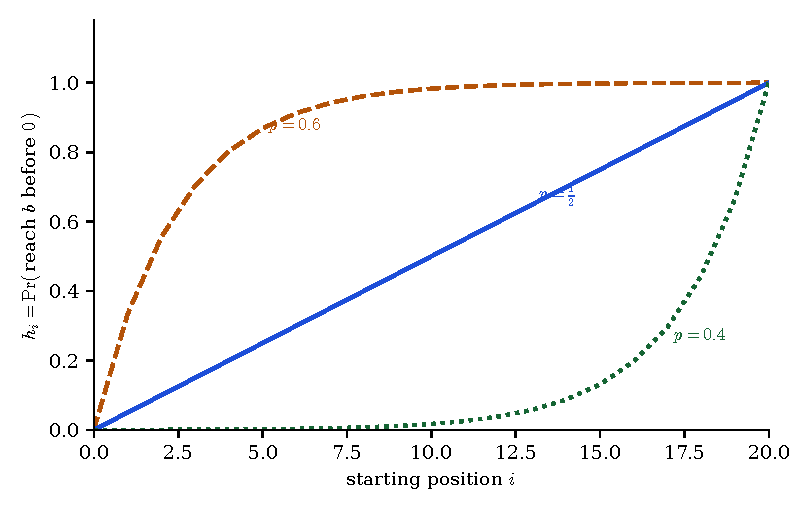
\includegraphics[width=0.86\textwidth]{figures/ruin_prob.pdf}
\caption{Hitting probabilities \cref{m:eq:ruinprob} of the gambler's ruin
problem with $b=20$: the probability $h_i$ of reaching $b$ before $0$ from
starting position $i$, for $p=0.4$, $\tfrac12$ and $0.6$. Drift towards the
target makes the probability rise steeply and saturate near one; drift away
from it confines the mass to the far end of the interval; the symmetric case
interpolates linearly. The same first-step difference equation, with
$q/p$ replaced by $\mu/\lambda$, is the continuous-time hitting probability of
\cref{m:eq:bdhitting}.}
\label{m:fig:ruin}
\end{figure}
